% !TEX root = ../a3.tex

\section{Introduction}
In this report, we discuss the time complexity of three types of different priority queues including \emph{Unsorted heap}, \emph{Binary heap} and \emph{Fibonacci heap}, by testing their average runtime applied in \emph{Dijkstra Single-Source-Shortest-Path Algorithm}. For each test case size, we have five distinct maps, testing the extreme situation where the source and sink locate on the diagonal of the map.

In the test case, the test code \con{\#define TEST} to hide all the unnecessary output part and obtain the direct runtime of \emph{Dijkstra Algorithm}.

It's noteworthy that since \emph{Dijkstra Algorithm} cannot deal with negative weight edges, the randomized weights for each grid is restricted to $[0, 100]$ to prevent the intermediate or final path cost from exceeding the limit of \con{int}.

\section{Performance analysis on Selection Algorithms}
\begin{figure}[H]
    \centering
    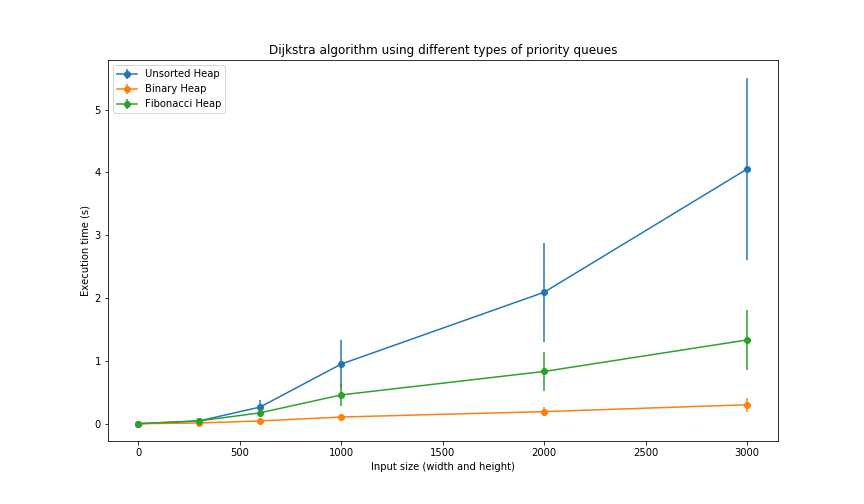
\includegraphics[width=0.75\linewidth]{../a3/test/res}
    \caption{Dijkstra algorithm using different types of priority queues}\label{res}
\end{figure}
To graphically demonstrate the outcome, here the standard deviation of tests are kept as error bar.

Theoretically, \emph{Fibonacci heap} take an edge over three of these three priority queues on amortized time complexity. The \con{enqueue} operation of \emph{Fibonacci heap} is $O(1)$ and the \con{dequeue\_min} operation of which is $O(\log n)$. Nevertheless, the runtime result does not manifest the advantage. \emph{Fibonacci heap} is much faster than \emph{Unsorted heap}, undoubtedly, runs clearly slower than binary tree in practice.

Presumably, the disappointment results, firstly, from the frequent memory operation and the construction of structures like \con{node\_t *} and \con{coord} (see Appendix). Thus, \emph{rvalue reference} is introduced here. If the memory operation is efficient, the power of \emph{Fibonacci heap} might boost. On the contrary, the binary tree only entails index accessing to the vector. The time cost is relatively small.

Moreover, the constant of the time complexity of \emph{Fibonacci heap} may be larger than \emph{Binary heap} because each operation of the former requires several memory steps. Also, if the root list in \emph{Fibonacci heap} accumulates, then the time complexity of \con{consolidate} may degrade to $O(n)$.


\section{Conclusion}
In this report, we have demonstrated the characteristics of three different priority queues applied in Dijkstra Algorithms as well as their performance. \emph{Unsorted heap} is essentially not a good way to maintain the minimum key value. Each time it requires a traversal to get the result. The interesting comparison between \emph{Fibonacci heap} and \emph{Binary heap} shows that the latter one outperform significantly. Theoretically, \emph{Fibonacci heap} seems better but in practice, \emph{Binary heap} is a better choice both on runtime and the difficulty to implement.

\clearpage
\section{Appendix}
\appendix
\section{Source Codes}
\inputcode{c++}{../a3/test/a3.cpp}{Dijkstra algorithms using three different heaps}{1}
\inputcode{python}{../a3/test/test.py}{Test case generator}{2}
\inputcode{bash}{../a3/test/test.sh}{Test case runner}{3}
\inputcode{python}{../a3/test/plot.py}{Plotting program}{4}